\documentclass{article}
\usepackage[utf8]{inputenc}
\usepackage{hyperref}
\usepackage[letterpaper, portrait, margin=1in]{geometry}
\usepackage{enumitem}
\usepackage{amsmath}
\usepackage{booktabs}
\usepackage{graphicx}
\usepackage{float}

\usepackage{hyperref}
\hypersetup{
colorlinks=true,
    linkcolor=black,
    filecolor=black,      
    urlcolor=blue,
    citecolor=black,
}
\usepackage{natbib}

\usepackage{titlesec}
  
\title{Homework 2}
\author{Lin Yang}
\date{\today}
  
\begin{document}
  
\maketitle
\section{Python}

\subsection{Check for balance between the treatment and control groups}

\begin{table}[ht]
	\centering
	\begin{tabular}{llll}
\toprule
{} &   Control &  Retrofit & Difference \\
{} &      Mean &      Mean &    p value \\
{} &    (s.d.) &    (s.d.) &  of t-test \\
\midrule
Electricity &   1181.33 &   1086.75 &      0.001 \\
            &  (454.31) &  (423.96) &            \\
Sqft        &   1633.05 &   1657.55 &      0.572 \\
            &  (682.90) &  (686.27) &            \\
Temp        &     79.89 &     79.89 &      0.987 \\
            &    (2.16) &    (1.97) &            \\
\bottomrule
\end{tabular}

	\caption{Summary Statistics by control and treatment group}
\end{table}
The characteristics of Sqft and Temp are good measures for the households since the p-values of the two variables in the t-test is large, which means that the average Sqft and Temp among two groups are similar. \\ And the p-value of Electricity is less than 1\%, which means there is significant difference in Electricity use between two groups and the randomized experiment succeeded in creating the desired variation.
	
\subsection{Kernel Density Plots}

\begin{figure}[ht]
	\centering
	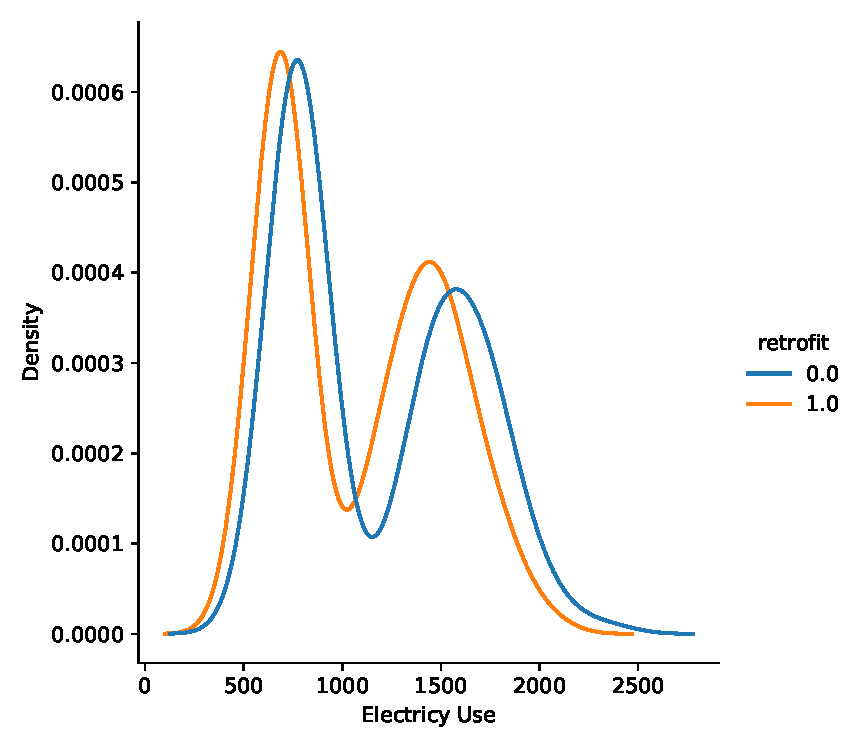
\includegraphics[scale = 0.5]{q2.pdf}
	\caption{Kernel density plots of electricity use by control and treatment group}
\end{figure}


\subsection{Estimation}

\textbf{(a) OLS by hand}
\begin{table}[ht]
	\centering
	\begin{tabular}{lr}
\toprule
{} & OLS (by hand) \\
{} &  Coefficients \\
\midrule
Constant &    -83.602758 \\
Sqft     &      0.615339 \\
Retrofit &   -109.666176 \\
Temp     &      3.255075 \\
\bottomrule
\end{tabular}

	\caption{Coefficients from calculating OLS by hand }
\end{table}

\textbf{(b) OLS by simulated least squares}
\begin{table}[ht]
	\centering
	\begin{tabular}{lr}
\toprule
{} &            OLS \\
{} &  (by simulated \\
{} & least squares) \\
{} &   Coefficients \\
\midrule
Constant &     -83.556600 \\
Sqft     &       0.615338 \\
Retrofit &    -109.666059 \\
Temp     &       3.254502 \\
\bottomrule
\end{tabular}

	\caption{Coefficients from simulated least squares}
\end{table}


\textbf{(c) OLS using a canned routine}
\begin{table}[ht]
	\centering
	\begin{tabular}{lr}
\toprule
{} &               OLS \\
{} &  (by StatsModels) \\
{} &      Coefficients \\
\midrule
Constant &        -83.602758 \\
Sqft     &          0.615339 \\
Retrofit &       -109.666176 \\
Temp     &          3.255075 \\
\bottomrule
\end{tabular}

	\caption{Coefficients from using a canned routine}
\end{table}


\section{Stata}

\subsection{Check for balance between treatment and control group.}

\begin{table}[H]
	\centering
	{
\def\sym#1{\ifmmode^{#1}\else\(^{#1}\)\fi}
\begin{tabular}{l*{3}{cc}}
\hline\hline
                    &\multicolumn{1}{c}{Control}&\multicolumn{1}{c}{Retrofit}&\multicolumn{1}{c}{Difference}\\
                    &     mean/sd&     mean/sd&           p         \\
\hline
electricity         &     1181.33&     1086.75&       0.001\sym{***}\\
                    &      454.31&      423.96&                     \\
sqft                &     1633.05&     1657.55&       0.572         \\
                    &      682.90&      686.27&                     \\
temp                &       79.89&       79.89&       0.987         \\
                    &        2.16&        1.97&                     \\
\hline
Observations        &         501&         499&        1000         \\
\hline\hline
\end{tabular}
}

	\caption{Summary Statistics by control and treatment group}
\end{table}


\subsection{Scatter Plot with electricity consumption vs sqft}
\begin{figure}[ht]
	\centering
	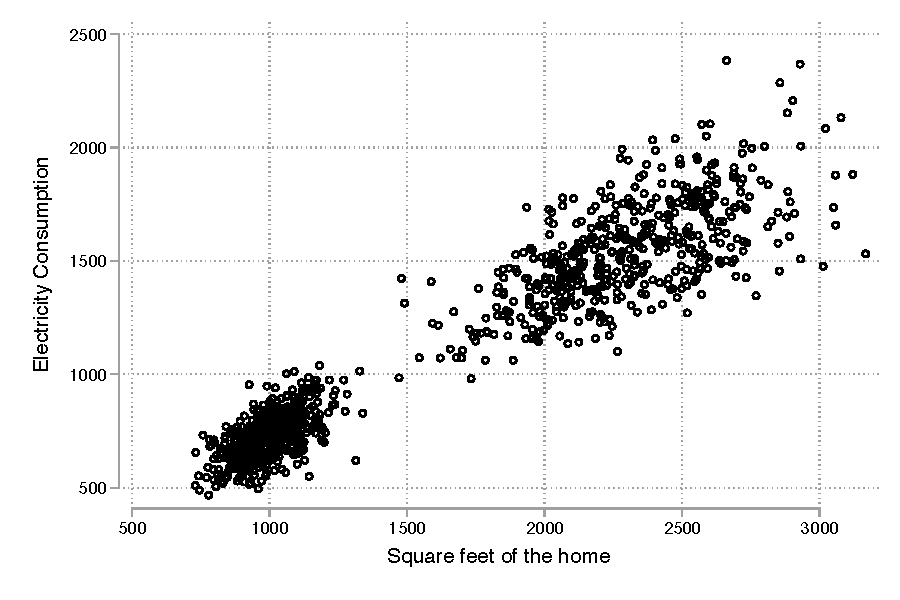
\includegraphics[scale = 0.7]{scatterplot.pdf}
	\caption{Scatter plot of electricity consumption versus square feet}
	\label{fig:scatterplot}
\end{figure}



\subsection{Regression Results}
\begin{table}[H]
\centering
	\begin{tabular}{lc} \hline
 & (1) \\
VARIABLES & Ordinary least squares \\ \hline
 &  \\
sqft & 0.62** \\
 & (0.01) \\
retrofit & -109.67** \\
 & (7.94) \\
temp & 3.26 \\
 & (1.93) \\
Constant & -83.60 \\
 & (154.69) \\
 &  \\
Observations & 1,000 \\
 R-squared & 0.92 \\ \hline
\multicolumn{2}{c}{ Robust standard errors in parentheses} \\
\multicolumn{2}{c}{ ** p$<$0.01, * p$<$0.05} \\
\end{tabular}

	\caption{Regression results table with heteroskedasticity standard errors}
\end{table}





\end{document}

